\documentclass[two column]{article}
\usepackage[utf8]{inputenc}

\usepackage{amsmath,amsthm,amssymb}

\usepackage{subcaption}
\usepackage{graphicx}

\usepackage{diagbox}

\graphicspath{{./images/}}

\usepackage{listings}


\usepackage{color}

\definecolor{gray}{rgb}{0.5,0.5,0.5}
\definecolor{orange}{rgb}{0.8,0,0}

\lstdefinestyle{matlab}{
  belowcaptionskip=1\baselineskip,
  breaklines=true,
  frame=L,
  xleftmargin=\parindent,
  language=octave,
  showstringspaces=false,
  basicstyle=\footnotesize\ttfamily,
  keywordstyle=\bfseries\color{green},
  commentstyle=\color{gray},
  identifierstyle=\color{blue},
  stringstyle=\color{orange},
}

\def\listingsfont{\ttfamily} 
\def\listingsfontinline{\ttfamily}

\title{TAMS39 - Examination exercises}
\author{Anton Karlsson\\antka388\\931217-7117}
\date{}
\begin{document}
\maketitle

\section*{Exercise 1}

\subsection*{(a)}
\label{sec:a}

Let $H_0: \b \mu_{\rm  male} = \b \mu_{\rm female}$ against $H_{1}: \b \mu_{\rm
  male} \neq \b \mu_{\rm female}$.
We get the test statistic $T^{2}$ which is given by
\begin{equation*}
  T^{2} = n(\mean X - \b \mu_{\rm male})^{T} S^{-1}(\mean X - \b \mu_{\rm male}),
\end{equation*}
where $\b S = \frac{1}{n-1}(\b X - \b 1\mean X^{T})(\b X - \b 1\mean
X^{T})^{T}$, $\b \mu_{\rm male} = (190, 275)^{T}$, and $n$ is the size
of the population. If $p$ is the dimension of the population, then 
\begin{equation*}
  \frac{n-p}{(n-1)p}T^{2} \sim F(p,n-p+1).
\end{equation*}
A test given by rejecting $H_{0}: T^{2} \geq \frac{(n-1)p}{n-p}F_{p,
  n-p}(1 -\alpha) = c_{\alpha}$, where $\alpha = 0.05$. We get that
$c_{\alpha} \approx 6.58$ and $T^{2} \approx 5.54
$, thus we cannot reject $H_{0}$.


\subsection*{(b)}
\label{sec:b}

The confidence region is given my all $\b \mu$ such that
\begin{equation*}
  n(\mean X - \b \mu)^{T}\b S^{-1}(\mean X - \b \mu) \leq \frac{(n-1)p}{n-p}F_{p,
  n-p}(1 -\alpha) = c_{\alpha}.
\end{equation*}
The result is displayed in Figure \ref{fig:ex1-ellipse}.
\begin{figure}[h]
  \centering
  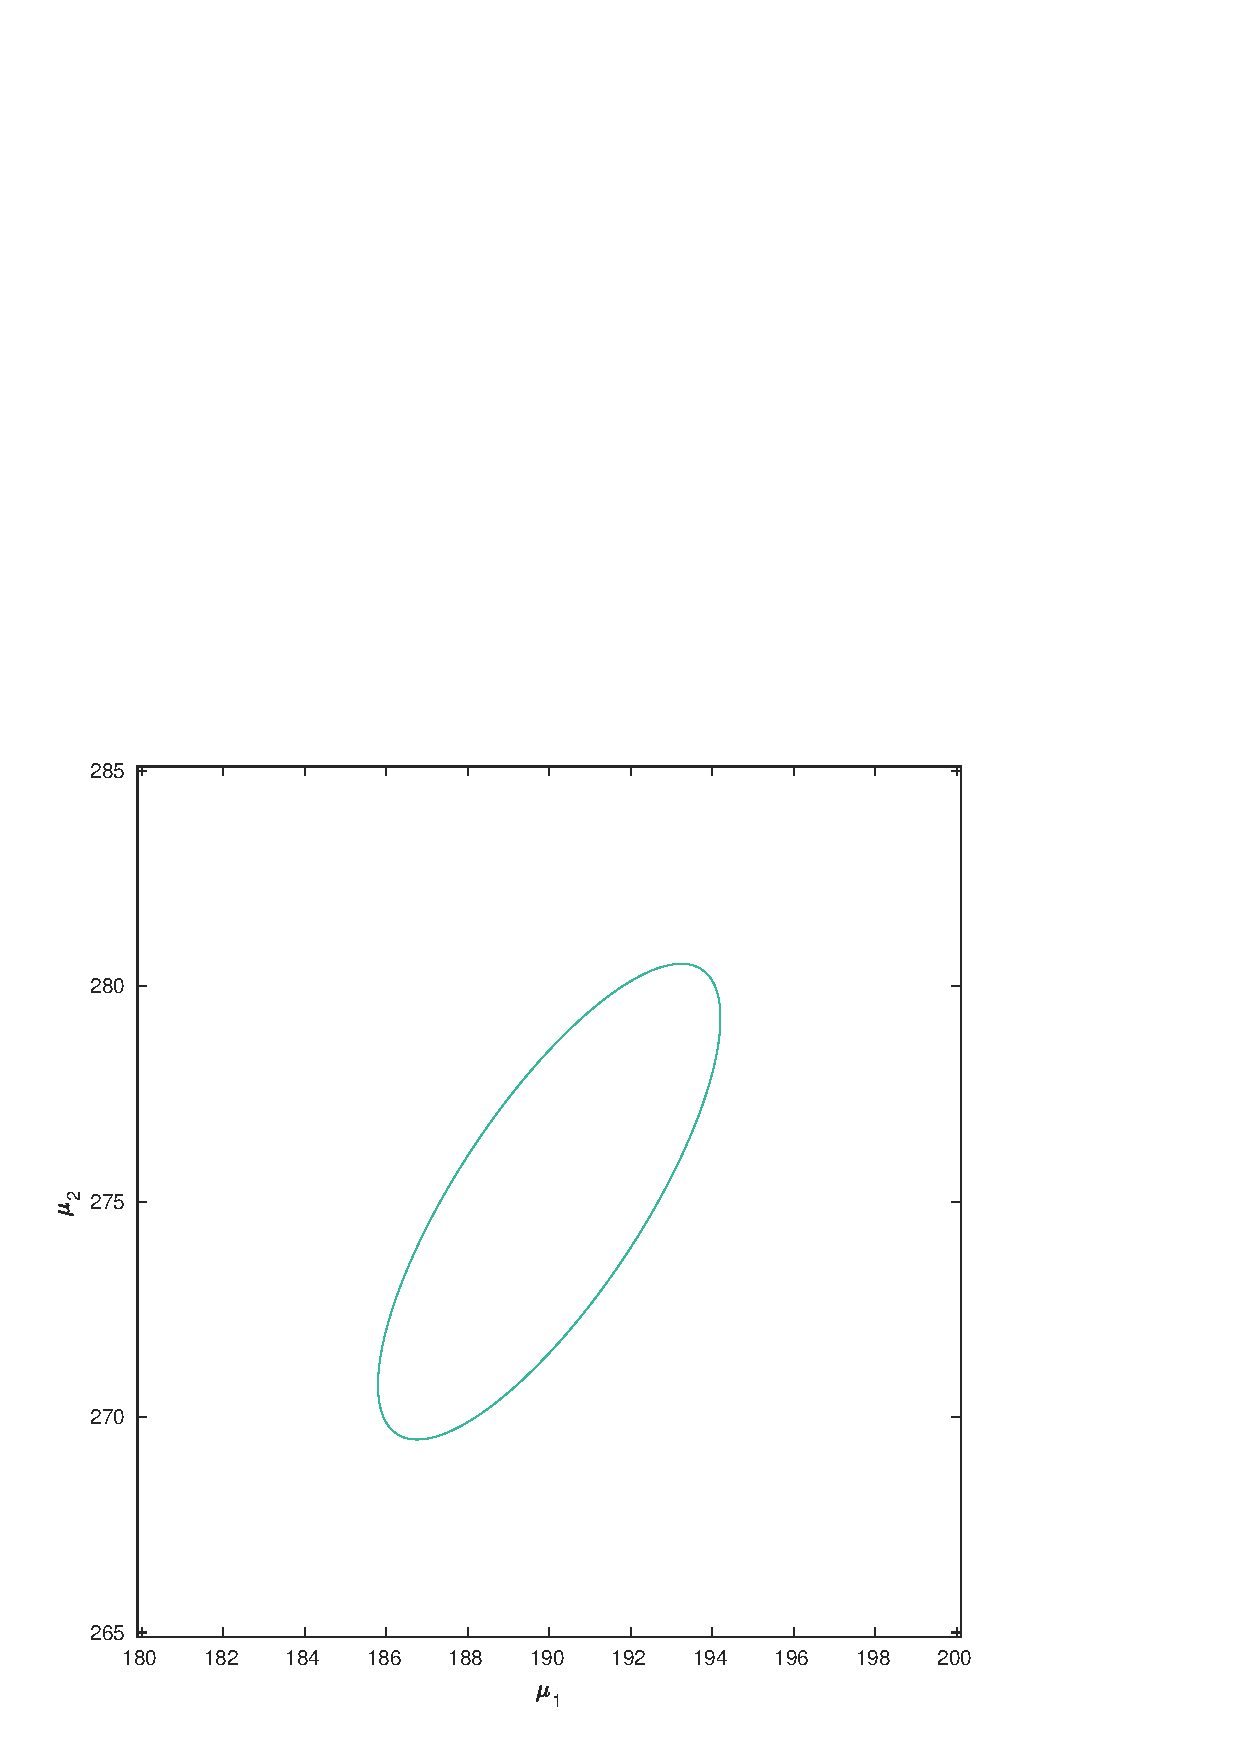
\includegraphics[width=5cm]{ellipse-ex1}
  \caption{The confidence ellipse around ${\bf \mu}$.}
  \label{fig:ex1-ellipse}
\end{figure}

\subsection*{(c)}
\label{sec:c}

From Result 5.3 in \cite[p. 225]{book} we get that simultaneously
confidence interval for $\b a' \b \mu$ is  given by
\begin{equation*}
  \b a^{T} \mean X - \sqrt{\frac{(n-1)p}{n(n-p)}F_{p,
  n-p}(1 -\alpha) \b a^{T}\b S\b a} \leq \b a^{T} \b \mu \leq 
\b a^{T} \mean X + \sqrt{\frac{(n-1)p}{n(n-p)}F_{p,
  n-p}(1 -\alpha) \b a^{T}\b S\b a} .
\end{equation*}
We get that for $\b a = (1, 0)^{T}$, which represents $\mu_{1}$, and for
$\b a = (0,1)^{T}$, which represents $\mu_{1}$, the confidence
intervals are
\begin{equation*}
  \begin{pmatrix}
    185.80 &194.20 
  \end{pmatrix},\quad \text{and} \quad
  \begin{pmatrix}
    269.48 &280.52  
  \end{pmatrix},
\end{equation*}
respectively.\\
\\
The Bonferroni intervals are given by 
\begin{equation*}
  \overline{x}_{i} \pm t_{n-1}(1 - \alpha/(2m) )\sqrt{\frac{s_{ii}}{n}},
\quad i = 1,2,
\end{equation*}
where $m= 2$ is the number of intervals. The intervals for
$\mu_{1}$ and $\mu_{2}$ are
\begin{equation*}
  \begin{pmatrix}
    186.20 &193.80 
  \end{pmatrix}, \quad \text{and}\quad
  \begin{pmatrix}
    270.00 &280.00 
  \end{pmatrix},
\end{equation*}
respectively.\\
\\
One advantage that the $T^{2}$-intervals have over the corresponding
Bonfferoni intervals is that the
Bonfferoni intervals are given by the inequaltiy
\begin{equation*}
  P\left(\text{the interval }\overline{x}_{i} \pm t_{n-1}(1 - \alpha/(2m)
  )\sqrt{\frac{s_{ii}}{n}}\text{ contains }\mu_{i},
\quad \text{for }i = 1,2,\right) \leq 1 - \alpha,
\end{equation*}
which the $T^{2}$-intervals do  not have; they have an equality
instead, meaning that the $T^{2}$-intervals can be more accurate than
the Bonfferoni intervals. 
%%% Local Variables:
%%% mode: latex
%%% TeX-master: "examination"
%%% End:


\end{document}
%%% Local Variables:
%%% mode: latex
%%% TeX-master: t
%%% End:
